\section{Background \& Motivation}
\label{sec:Motivation}

\autoref{fig:MT} (left) depicts the various components of (a simplified, unary) MT. 
An input model $\mathsf{M}_{_{\mathsf{in}}}$, conforming to a source metamodel 
$\mathsf{MM}_{_{\mathsf{src}}}$, is transformed into an output model 
$\mathsf{M}_{_{\mathsf{out}}}$, hopefully conforming to a target metamodel
$\mathsf{MM}_{_{\mathsf{tgt}}}$, by the execution of an MT specification.

\begin{figure}[t]%
   \begin{minipage}[t]{0.46\columnwidth}
      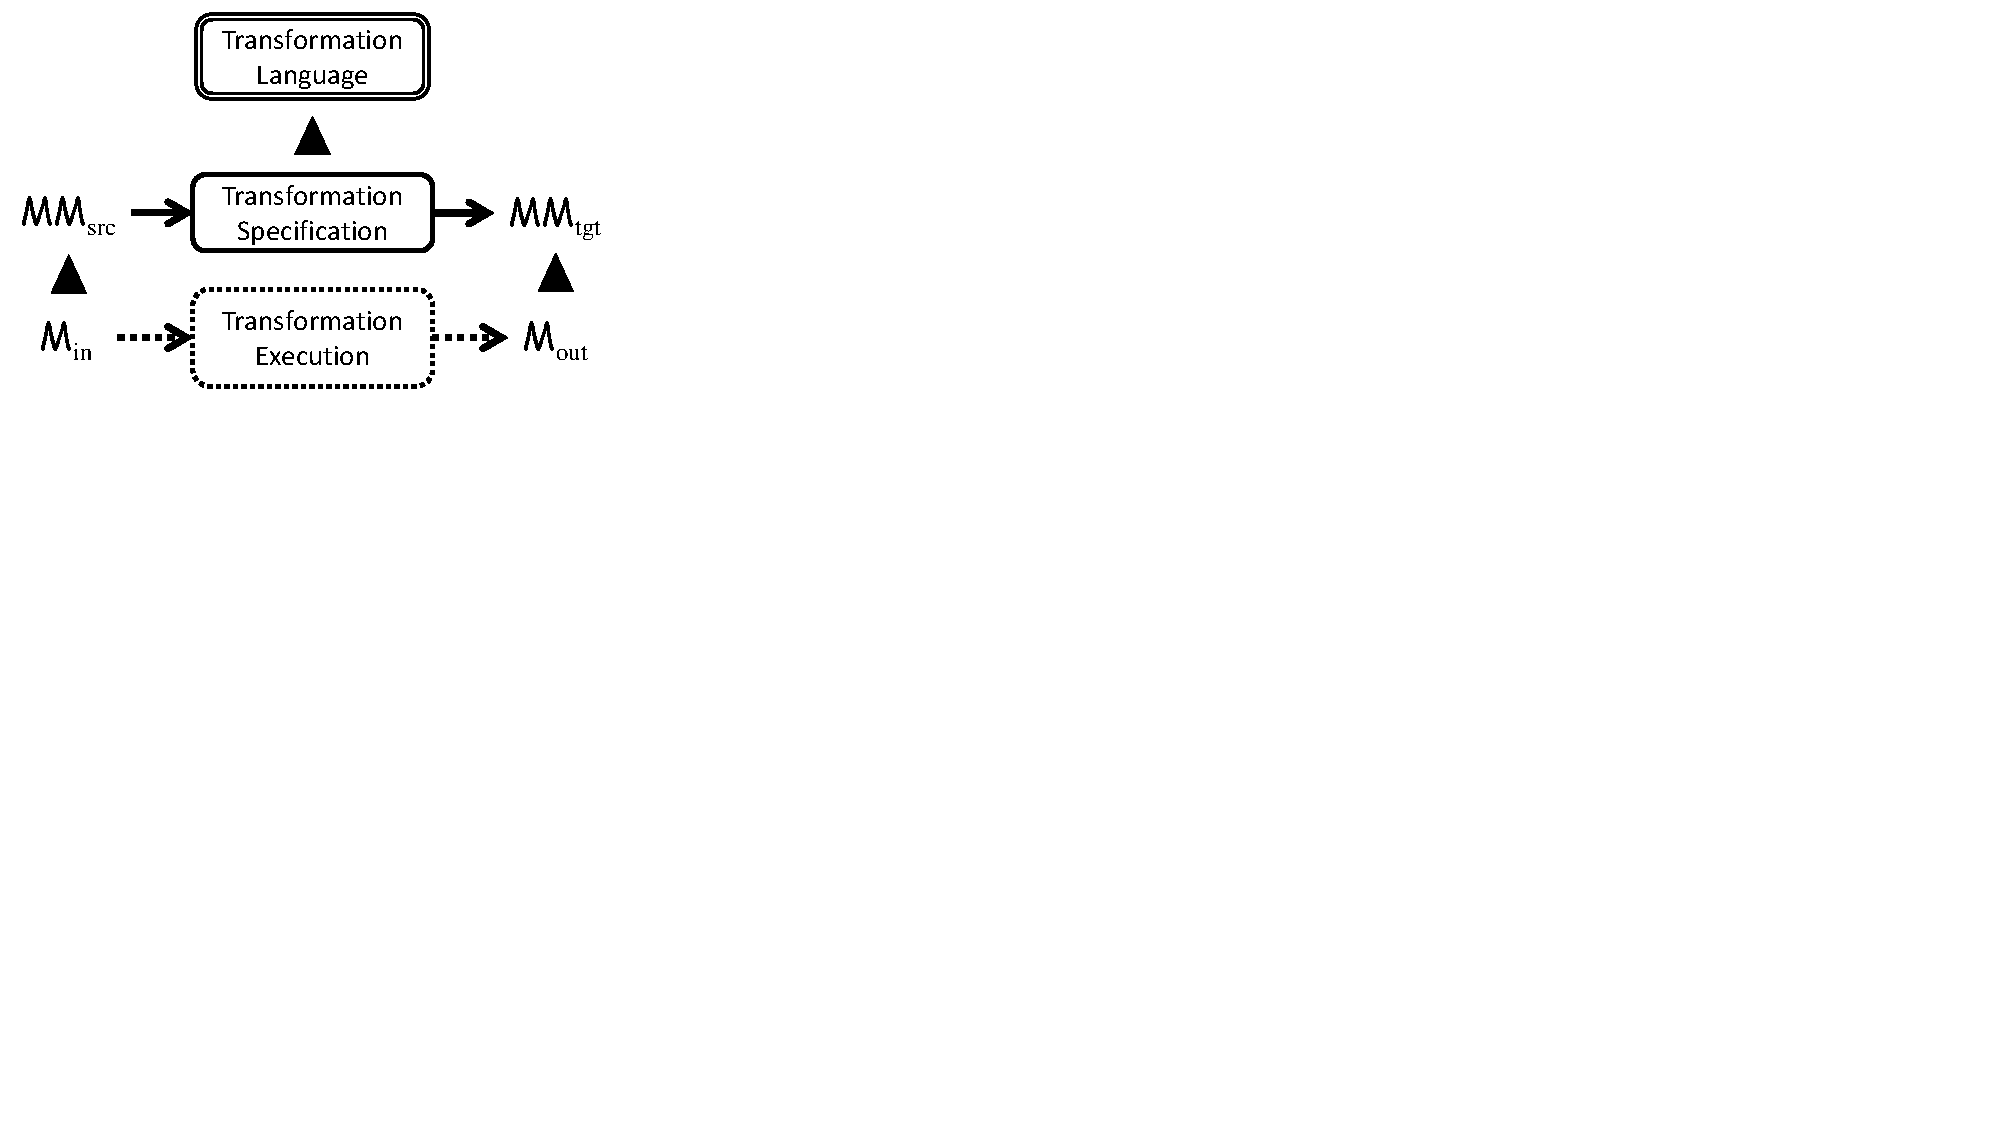
\includegraphics[width=\columnwidth,page=1,clip, trim=0.3cm 12.5cm 23.5cm 0.2cm]{ModelTransformation.pdf}
   \end{minipage}
   \hfill
   \begin{minipage}[b]{0.53\columnwidth}
   \includegraphics[width=\columnwidth,page=2,clip, trim=0.5cm 13.7cm 23cm 0cm]{ModelTransformation.pdf}%
   \end{minipage}
   \caption{Model \emph{Transformation} (MT) (left) and Model \emph{Animation} (MA),
   as a special case of MT, operating on the \emph{concrete syntax} of model $\mathsf{M}$,
   which is involved in an endogenous, in-place \emph{simulation} MT. Metamodels
   $\mathsf{MM}$ and $\mathsf{MM}_{\mathsf{CS}}$ may be related through rendering/parsing}%
   \label{fig:MT}%
   \Description[<short description>]{<long description>}
\end{figure}


MTs are not created equal: whereas they may seem syntactically, and sometimes 
semantically, similar, they may serve different purposes (known as MT intents
\citep{J:Lucio-Amrani-etAl:2014} in the literature) that need to be adequately
distinguished. For the purpose of this paper, three different MT intents are
interesting to precisely define, because they often raise confusion in the literature.
For an input model \textsf{M},
\begin{description}
   \item[Visualisation] is an intent characterising an outplace, heterogeneous
   MT aiming at visually \emph{representing}, or \emph{rendering}, \textsf{M} 
   through the definition of a \emph{visual} concrete syntax mainly composed of 
   graphical symbols.
   
   \item[Simulation] is an intent characterising an inplace, endogeneous MT aiming
   at defining \textsf{M}'s operational semantics, i.e. how \textsf{M} evolves 
   over time during execution.
   
   \item[Animation] is ``\emph{the visual representation of a simulation}'' 
   \citep{J:Lucio-Amrani-etAl:2014}, i.e. it visually renders the computation steps
   defined by the MT simulation specification, by visually projecting the changes
   operated on the simulated model through its (visual) concrete syntax.
\end{description}
Summarising, an \emph{animation} is tightly connected to a \emph{simulation} through
the use of a(n existing) \emph{visualisation}.
In other terms, designing an MA requires the following components, as depicted 
in \autoref{fig:MT} (right):
\begin{itemize}
	\item A Concrete Syntax \textsf{CS} that should be defined over \textsf{MM}, so
   that it becomes possible to \emph{visualise} \textsf{M} as a graphical model 
   $\mathsf{M}_{\mathsf{CS}}$.
   
   \item \textsf{MM}'s operational semantics is specified in a \emph{simulation}
   MT (specification).
   
   \item \emph{during} each run of the simulation's execution, the computing steps
   are visually rendered over $\mathsf{M}_{\mathsf{CS}}$.
\end{itemize}

Just like MTs are built over transformation \emph{units}, i.e. basic building blocks
that are composed to realise larger, complex transformations, it is likely that 
MA requires a similar decomposition process into basic ``units'' to build and 
organise them. However, MTs are likely specified independently of any MA, primarily
for capturing the \DSL's behaviour, but also likely for supporting other activities
(typically, code generation, and various analyses, among others). Since both an MT
and an MA for a given model \textsf{M} exist for different purposes, it seems 
reasonable to build them separately, and even to entrust their specification to
different persons, or teams, thus creating a new \emph{role} in \MDE: the 
\emph{MA Designer}, who need adequate methodologies and tools to perform the job.

Although serving different concerns, MT and MA are by nature tightly connected,
since they both encode a \DSL's behaviour. A Model Transformation Unit (TU) is the
smallest, coherent unit of computation visible from the outside. An interesting
approach would consist in directly relating, or connecting, the (execution of) a
Model Animation Unit (AU) to (the execution of) a TU, so that the changes performed
inside the TU are visually rendered. 

However, to fully unlock the potential of MA engineering, the specification of AUs
should be completely decoupled from the specification of (and languages for) TUs.
As they serve a common purpose, a mechanism for explicitly relating AUs to corresponding
TU(s) is required for this vision to work: when the execution engine of the MTL
executes a TU, it passes information to the MA engine to concurrently run the
animation. This vision is directly inspired by existing methodologies for designing 
debuggers for MTLs \citep{bousse2018omniscient,J:VanMierlo-Vangheluwe-etAl:2020}:
to avoid inspecting models that may be inconsistent during the execution of a TU,
a so-called debugging \emph{step} is defined by annotating TUs relevant for inspection.
An execution \emph{step} provides the support for animation steps.

Conceptually, TUs and AUs should be in an \textsf{N:N} relationship, as depicted
in \autoref{fig:TU-AU}
\begin{itemize}
	\item A TU may be connected to several AUs, in order to provide different abstraction
   levels, and multiple views on the same execution (part). Typically, a beginner
   may need detailed visual information to understand a specific part of a model's
   execution, while a more advanced user may be happy with minimal animation. We
   illustrate this by providing several animations for typical \DSLs in \S \ref{sec:Examples}.

   \item An AU may be connected to many, but different, TUs, likely integrated in simulations
   for different models. Associated with appropriate composition operators, this
   approach promotes the definition of AUs libraries that capture popular and 
   widely used animation \emph{patterns}, thus enabling modularity and reuse 
   across \DSLs. We show in \S \ref{sec:Param} how similar AUs may be reused for
   rendering different MTs.
\end{itemize}

\begin{figure}[t]%
   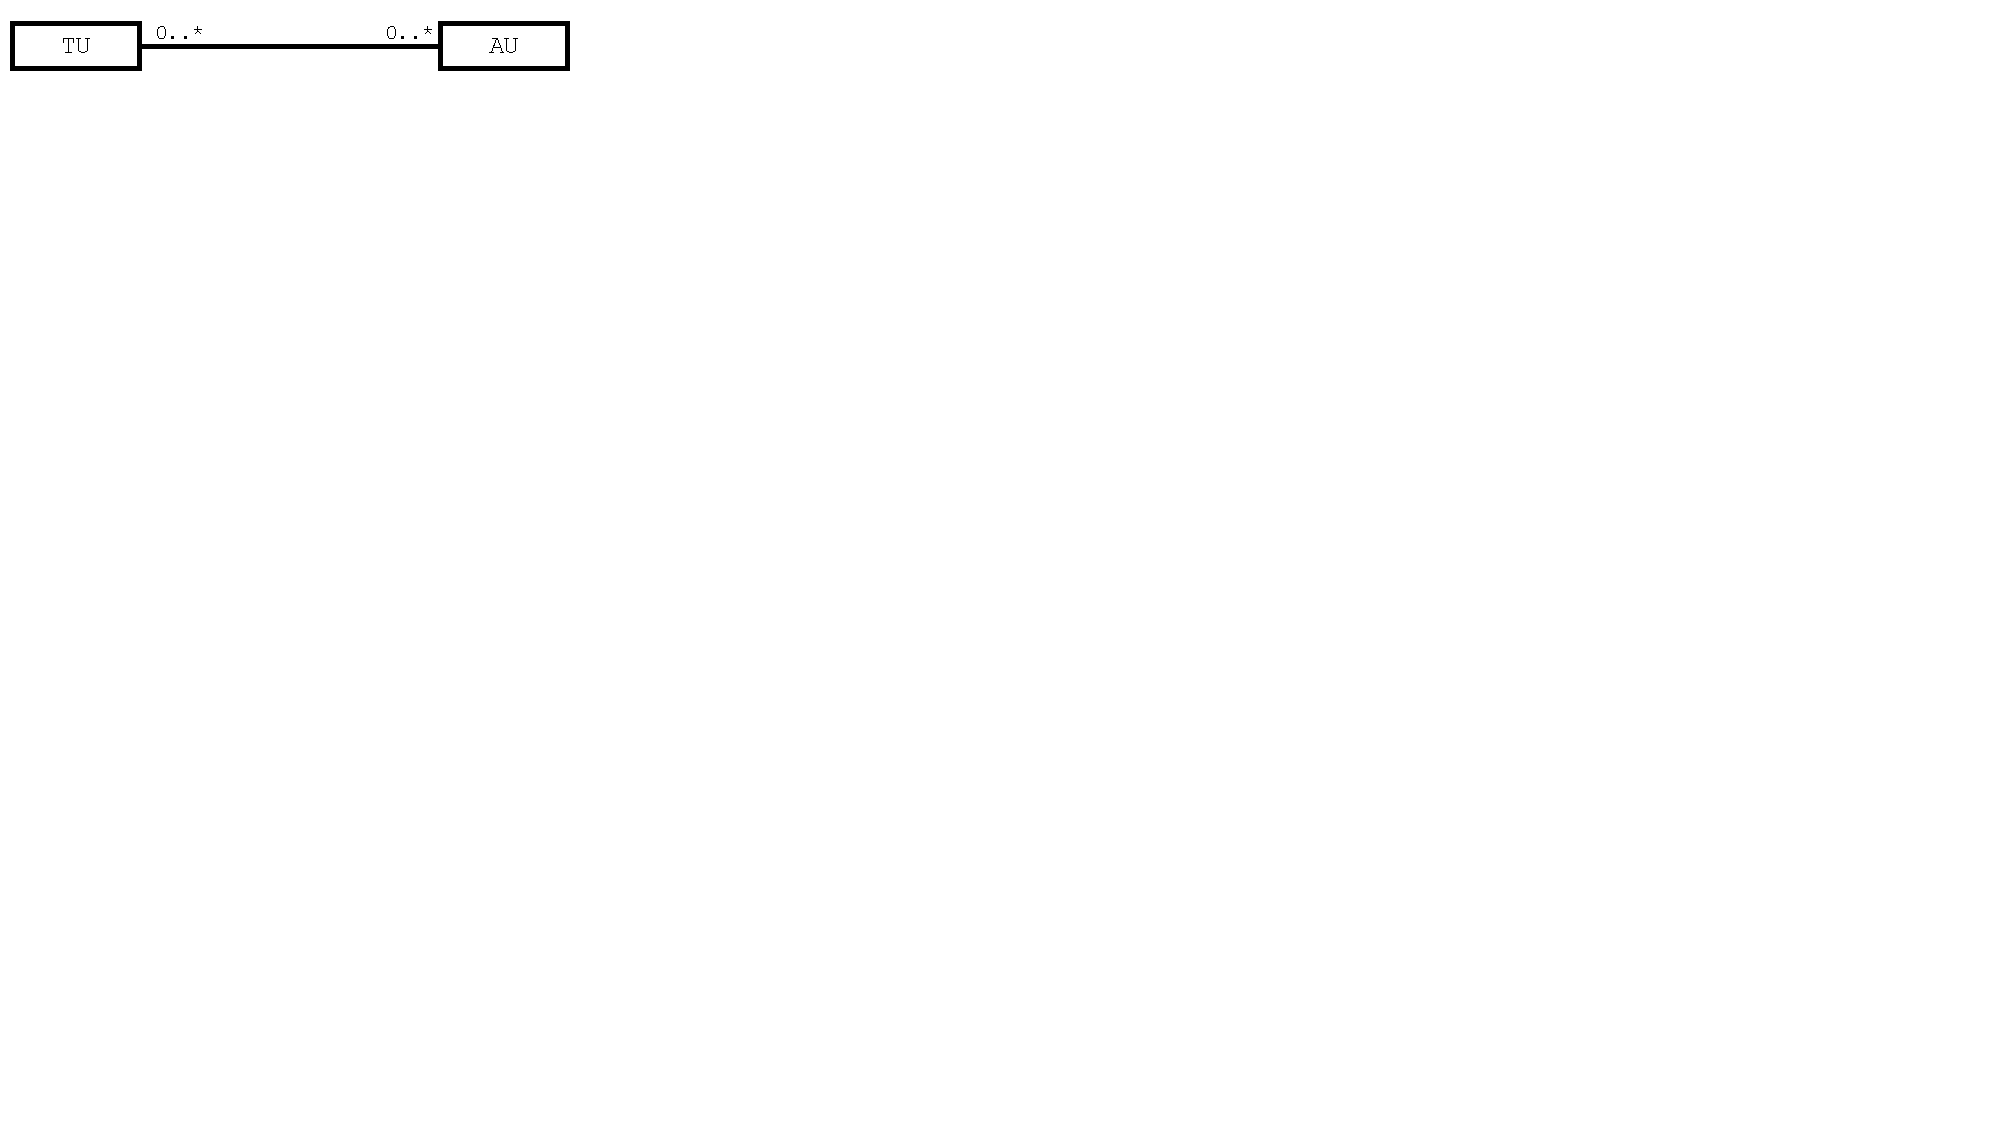
\includegraphics[width=\columnwidth,clip, trim=0cm 17.8cm 24.2cm 0.2cm]{TU-AU}%
   \caption{Relationship between Transformation (TU) and Animation (AU) Units for
   promoting multi-abstraction, and reuse.}%
   \label{fig:TU-AU}%
   \Description[Relating Transformation Units with Animation Units]{%
   For promoting multi-abstraction and reuse, Transformation Units (TUs) are in
   a N:N relationship with Animation Units (AUs).
   }
\end{figure}

To summarise our vision for enabling a systematic design of MA, we assume that a 
\DSL Engineer has already defined the core components, i.e. a metamodel capturing
the abstract syntax, one concrete syntax allowing to create, edit and manage 
conforming models, and a simulation that captures the \DSL's behaviour, specified
in an MTL that defines identifiable TUs. The missing steps, and corresponding challenges,
for an MA Engineer, would be the following:

\begin{description}
   \item[C1.] How to explicitly model a Concrete Syntax, with sufficient details
   to support animation? Since MA basically consists of continuously updating the
   concrete syntax of a \DSL along its execution, an explicit representation of the
   concrete syntax that exposes the graphical features to the MA designer is 
   required.
   
   \item[C2.] How to explicitly model an MA \emph{compositionally}, i.e. by creating an
   MA using basic components that are progressively composed in a fully-fledged
   animation? 
   
   \item[C3.] How to abstract away from the peculiar details of a given \DSL, thus
   promoting \emph{reuse}, and to explicitly map TUs with their related AU(s), to
   support \emph{flexibility}?
\end{description}
